\documentclass[../../paper.tex]{subfiles}
\begin{document}
\section{Research Data}
\subsection{Corpus}
The dataset we used for this research consists of $1.391.543$ articles from $3.759$ journals, all articles have been published in journals in 2017, that have (in 2017) at least 150 publications. Details about the corpus can be found in table~\ref{table:corpusSize}. The distribution of the text in our dataset follows a Pareto-like distribution, which is a common property of texts (\citet{wiegand2018word}). Our word and token distribution is visualized in Figure~\ref{figure:wordTokenOccurrence}, which displays the occurrences of the first 500 tokens and words of the corpus, ordered on occurrences.
\FloatBarrier
\begin{table}[hbt]
\begin{center}
\begin{tabular}{|l|r|r|r|}
\hline
 & Total count & Unique count & Average length\footnotemark \\
\hline\hline
Title words & $18.822.399$ & $939.665$ & 14  \\
\hline
Title tokens & $14.742.192$ & $230.805$ & 11 \\
\hline\hline
Abstract words & $264.653.020$ & $5.853.077$  & 190  \\
\hline
Abstract tokens & $171.474.473$ & $738.961$ & 124 \\
\hline\hline
Total words & $283.475.419$ & $6.209.769$  & 204 \\
\hline
Total tokens & $186.962.354$ & $763.475$ & 135 \\
\hline
\end{tabular}
\end{center}
\caption{Corpus size}\label{table:corpusSize}
\end{table}
\FloatBarrier
\footnotetext{Rounded}
\FloatBarrier
\begin{figure}[hbt]
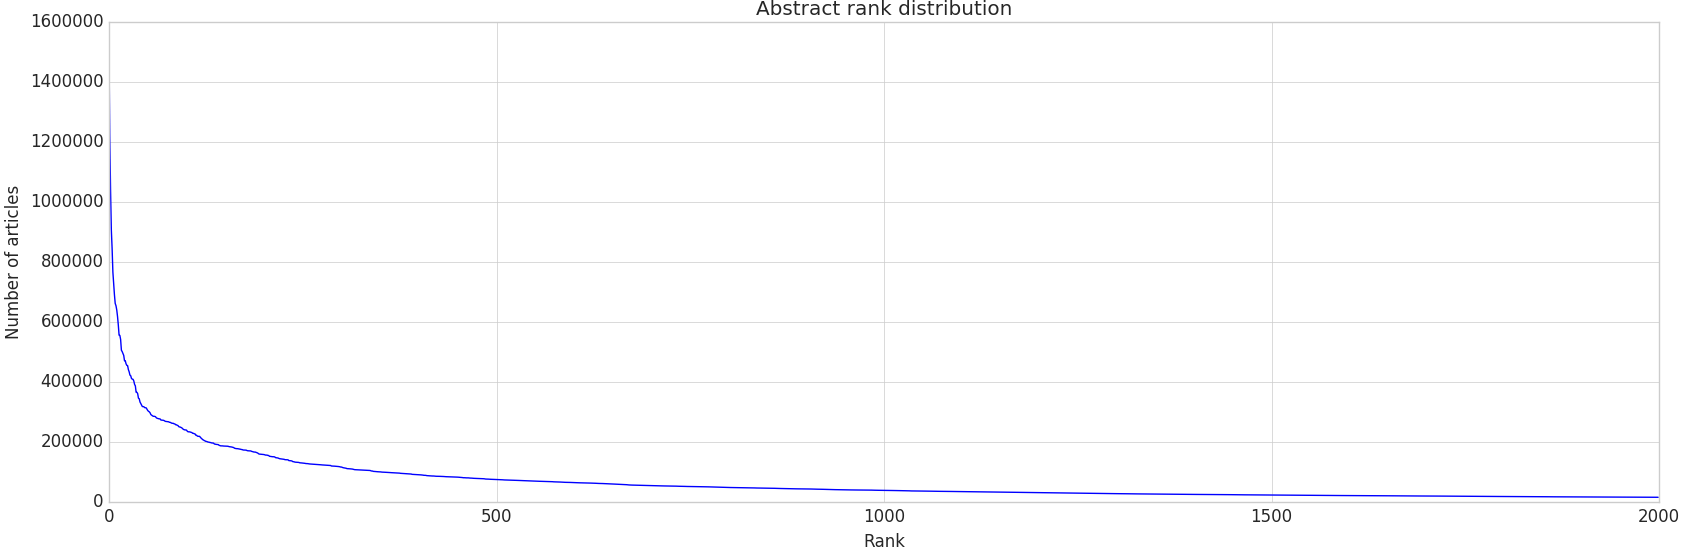
\includegraphics[width=4.5in]{Plots/word_occurrences}
\caption{Word and token occurrences. The y-axis shows the number of occurances for each word/token, the x-axis shows the occurence rank of the word/token; the position of the word/token in a list sorted on occurance.}\label{figure:wordTokenOccurrence}
\end{figure}
\FloatBarrier
\subsection{Datasets}
For this research we used a tokenized dataset, created from the earlier described corpus (see table~\ref{table:corpusSize}). From this tokenized set, we created the embeddings and the TF-IDF feature vectors. The following steps have been applied to convert the words from the text to tokens: removing punctuation, non-ascii characters, number \& stop-words, transforming all characters to lower-case and by stemming all remaining tokens using the NLTK stemmer\footnote{Natural Language ToolKit library, \url{https://www.nltk.org/}.}.
These steps reduced our dataset by 34\% (words to tokens), resulting in a set of $186.962.354$ tokens.
\subsubsection{Embedding}
For this research, we reused the word embeddings created by \citet{Truong2017Thesis}. These embeddings have a vector dimension of 300, and have been trained on the entire Elsevier corpus (titles and abstracts respectively), not limited to the subset we used for this research. To create higher-level embeddings, we average all component embeddings. Thus, to create article embeddings (higher level), we take the average of all normalized word embeddings (component) for that article. Journal embeddings are created by taking the average of all normalized article embeddings. We use the average to combine multiple embeddings into one because we determine the meaning of a larger text for this research as the "average meaning" of all components. We have used multiple embedding variations for this research. \textbf{Default embedding}; the embeddings  obtained from the word embeddings are referred to as the default embedding, \textit{embedding} in figures. A variation on this embedding is the \textbf{TF-IDF weighted embedding}. The word embeddings in this set have been weighted with the TF-IDF value for each word, we refer to this set as TF-IDF embedding, \}.{tfidf\_embedding} in figures. The TF-IDF score is calculated using the raw token count and the smoothed inverted document frequency. The \textbf{10K TF-IDF embedding} uses the TF-IDF embedding as basis, The 10K TF-IDF embedding set has been weighted with the same TF-IDF, but is limited to the top 10.000 most occurring tokens. This set is referred to as 10K TF-IDF embedding, \textit{10K\_embedding} in the figures. Another variation on the TF-IDF set is the \textbf{5K TF-IDF embedding}. The 5K TF-IDF embedding has also been weighted with the TF-IDF values, but has been limited to the top 5.000 most occurring tokens. This set is referred to as 5K TF-IDF embedding, \textit{5K\_embedding} in the figures. The \textbf{1K-6K TF-IDF embedding} set weights the word embeddings with the TF-IDF values and is limited to the tokens between the top 1.000 and top 6.000 based on their occurrence. Creating a set of 5.000 tokens, without using the top 1.000 tokens. We refer to this set as \textit{1k\_6k\_embedding} in the figures.
\subsubsection{TF-IDF}
The TF-IDF feature vectors are created using the TF-IDF model and a hasher from the PySpark MlLib\footnote{\url{http://spark.apache.org/docs/2.0.0/api/python/pyspark.mllib.html}.}.The TF-IDF feature vectors are created by hashing the tokens with the hasher, which has a set hash bucket size. These hashed values are passed on to the TF-IDF model, resulting in a feature vector with a dimension equal to the amount of hash buckets. To limit the computational and storage expenses and to reduce noise by rare words, we limit our vocabulary size. We label the TF-IDF configurations as follows: $vocabulary size/hash bucket size$. Furthermore, we denote 1.000 as 1K, since we deal with chosen values which can be exactly noted given this notation. This means that the set with a 10.000 vocabulary size and a 10.000 hash bucket size will be denoted as "10K/10K". We will refer to the TF-IDF configurations in our figures as "tfidf\_vocabulary size\_hash bucket size". Figure~\ref{figure:tfidfPerformance} shows the performance of TF-IDF on title and abstract as median rank, and Figure~\ref{figure:tfidfMemory} shows the storage size in gigabyte, of the 1k/1K, 4K/4K, 7K/7K and 10K/10K TF-IDF configurations. These figures show that, while the required storage size stagnates, the performance on title also quickly stagnates; the performance of the abstracts show similar behaviour. The stagnation of the storage size is likely due to the fact that the terms which are added to the larger vocabulary sets occur less often than the other words (the cut-off is based on word occurrence, descending). Given this information, we have chosen to use the 10K/10K, 10K/5K and 5K/5K configurations to compare our embedding results to because these configurations can be kept in memory (storage size) while it is not likely that larger sets will give much improvement. The TF-IDF feature vectors are created on article level and we average the set of article feature vectors to create a journal feature vector, just as we did with the embeddings.
\section{Pipeline}
\textbf{Data processing;} The research has been done in a python-databricks environment, which used Spark SQL, a library that offers tools to work with big-data. We processed the TF-IDF sets and the embedding sets \footnote{See Chapter 3.2 Datasets.} via the same pipeline, using their common vector properties. The pipeline contains the following steps: creating a training and validation set, creating the journal embeddings from the training set, categorizing the validation set articles using the journal embeddings and calculating the performance metrics.
\begin{figure}[hbt]
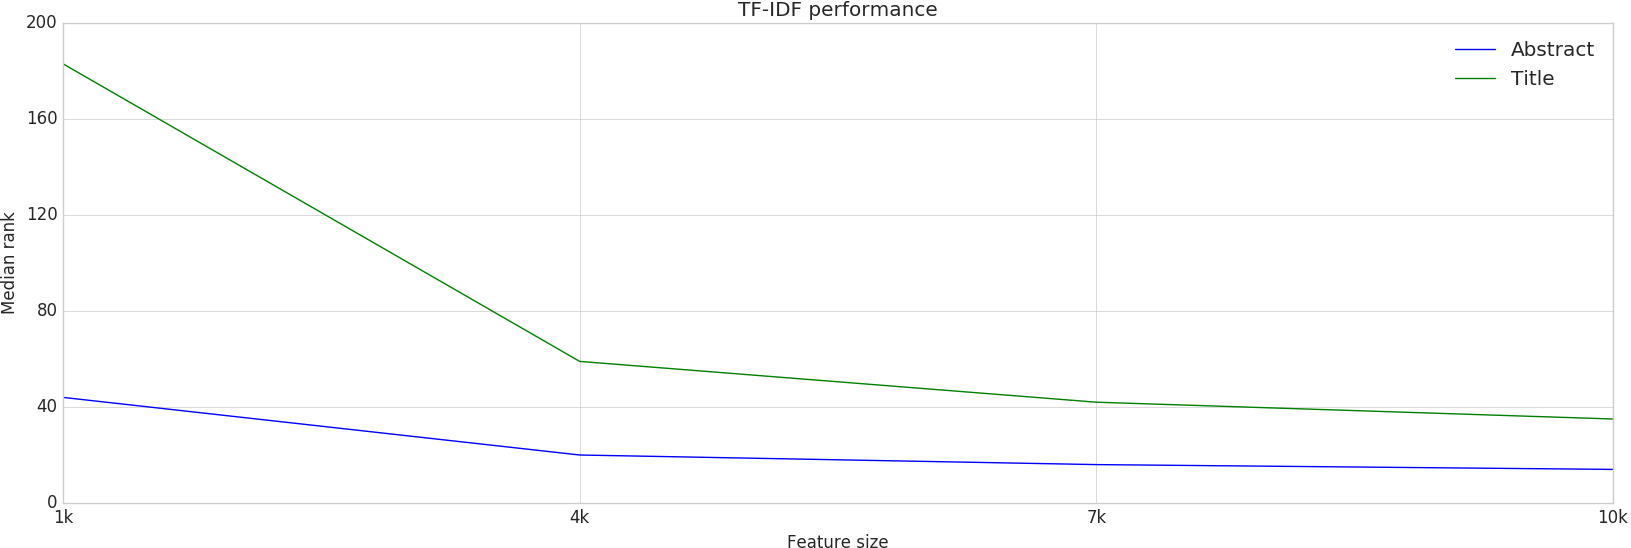
\includegraphics[width=5in]{Plots/tfidf_selection_plot_performance}
\caption{TF-IDF performance on title and abstract.}\label{figure:tfidfPerformance}
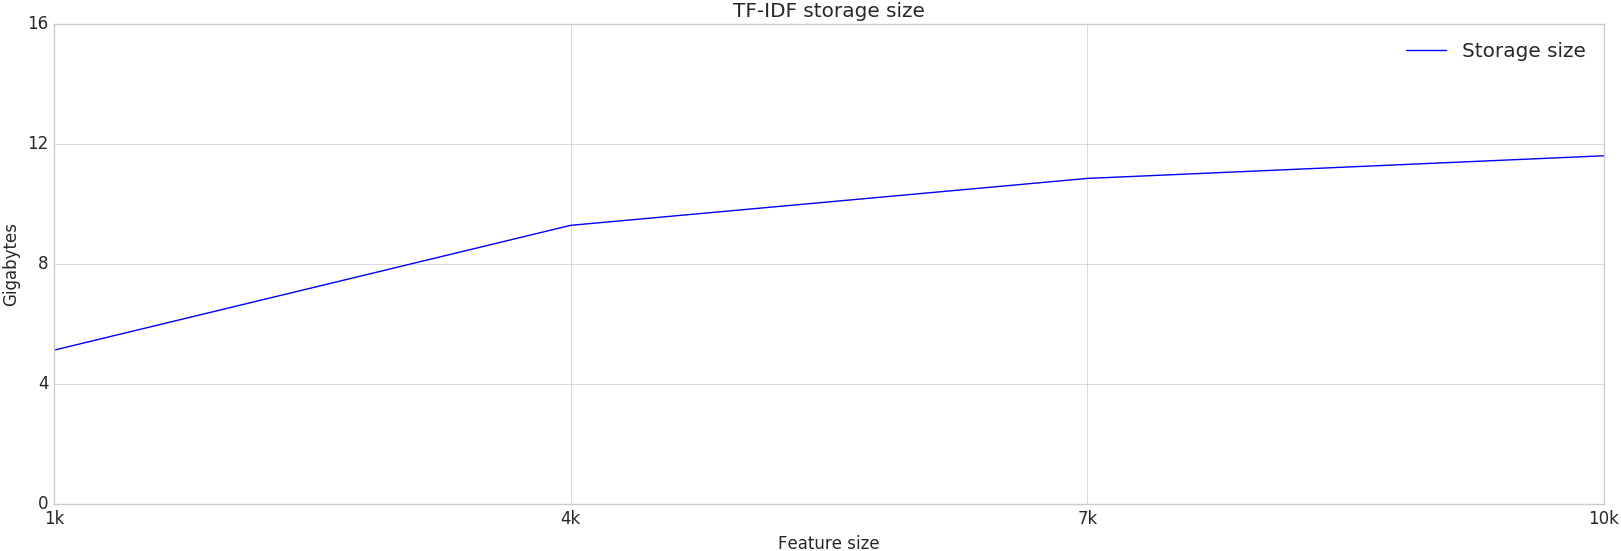
\includegraphics[width=5in]{Plots/tfidf_selection_plot_memory}
\caption{TF-IDF memory usage for title and abstract combined.}\footnote{We combined the memory usage of the titles and abstracts since the titles and abstract are created together and share their feature vector size.}\label{figure:tfidfMemory}
\end{figure}
\begin{itemize}
\item{Create training and validation set;
We split our initial set in a training set ($80\%$) and a validation set ($20\%$). This split of the data is based on a random number given to each article, ensuring that all datasets (i.e. tfidf\_10k\_10k, embedding) have the same (random) training and validation set.}
\item{Create journal embeddings;
From our training set we create the journal embeddings, which are created for most sets\footnote{See chapter 3.2 Datasets.} by averaging the article embeddings or feature vectors.}
\item{Categorize validation articles;
To categorize the articles, we calculate the distance between the title of the article (validation set), and the title of each journal (training set). We also do this for the abstract of the article and the abstract of each journal. During this process we record of the title-based-rank and abstract-based-rank of the source journal, best scored journal on abstract and title and the similarity between the source journal and article for both abstract and title.}
\item{Distance metrics;
To calculate the distance between two vectors, cosine similarity is commonly used. We validated the quality of cosine similarity as a distance metric by comparing it to other similarity metrics available in the SciPy library\footnote{\url{https://www.scipy.org/}}. We calculate the similarities based on the normalized embeddings, and compared the distance metrics based on the default embedding set. Table~\ref{table:distanceMetrics} shows the results of this validation.}
\end{itemize} 
\begin{table}[hbt]
\begin{tabular}{|l|r|r|r|r|}
\hline
Metric\footnotemark & Median title rank & Average title rank & Median abstract rank & Average abstract rank  \\
\hline
Braycurtis & 28 & 130 & 23 & 124  \\
\hline
Canberra & 33 & 148 & 26 & 133  \\
\hline
Chebyshev & 57 & 256 & 41 & 191  \\
\hline
\textit{Cityblock} & \textit{28} & \textit{130} & \textit{23} & \textit{124}  \\
\hline
\textit{Correlation} & \textit{27} & \textit{127} & \textit{23} & \textit{122}  \\
\hline
\textbf{Cosine} & \textbf{27} & \textbf{127} & \textbf{23} & \textbf{122}  \\
\hline
\textit{Euclidean} & \textit{27} & \textit{127} & \textit{23} & \textit{122}  \\
\hline
Mahalanobis & 136 & 544 & 75 & 449  \\
\hline
\textit{Seuclidean} & \textit{27} & \textit{124} & \textit{22} & \textit{115}  \\
\hline
\textit{Sqeuclidean} & \textit{27} & \textit{127} & \textit{23} & \textit{122}  \\
\hline
\end{tabular}
\begin{center}
\caption{Distance metric performance for word embeddings on the categorization of academic texts, only showing relevant results.}\label{table:distanceMetrics}
\end{center}
\end{table}
\footnotetext{As defined and provided by the SciPy library} 
The results in Table~\ref{table:distanceMetrics} show high similarity between cosine-based metrics (Cosine \& Correlation) and euclidean based metrics (Euclidean, Seuclidean \& Sqeuclidean). This similarity is expected, since the cosine and euclidean distances should yield the same results on normalized sets\footnote{See: \url{https://en.wikipedia.org/wiki/Cosine_similarity\#Properties}.}. The results show that some enhancement on the euclidean algorithm (Seuclidean) result in slightly improved results, although not significant. Also the Cityblock metric yields results close to the Cosine metric, only having a slightly worse performance, which is also not significant. Because of this, we will use the cosine-similarity as the distance metric, which will make our results easier to compare with other work, since the cosine-similarity is a commonly used similarity measure.
\subsection{Performance measurement}
We use multiple metrics to validate the performance of the embedding sets and TF-IDF sets on the categorization task. These metrics are: the F1-score, the Median \& average rank and the Rank distribution.
\begin{itemize}
\item{F1-score;
For our matching algorithm, we classify the results as follows:
$True Positive = $ Articles correctly matched to the current journal\\
$False Positive = $ Articles incorrectly matched to other journals\\
$False Negative = $ Articles incorrectly matched to the current journal\\
With these definitions, we calculate the Recall, Precision \& F1 using the standard formulas.}
\item{Median \& average rank;
We use both average and median ranks as rank-indication for a journal. The median rank indicates at which point 50\% of all values is larger and 50\% of all values is smaller, indicating the "typical article". While the average indicates the exact average of all articles in the set. We used both measures for our research.}
\item{Rank distribution;
To further analyse the ranking results, we plot the article rank distribution to get an indication of the ranking-landscape.}
\end{itemize}
\end{document}